\documentclass[
11pt, % The default document font size, options: 10pt, 11pt, 12pt
%codirector, % Uncomment to add a codirector to the title page
]{charter} 


% El títulos de la memoria, se usa en la carátula y se puede usar el cualquier lugar del documento con el comando \ttitle
\titulo{Evaluador de microcontroladores para misiones espaciales} 

% Nombre del posgrado, se usa en la carátula y se puede usar el cualquier lugar del documento con el comando \degreename
%\posgrado{Carrera de Especialización en Sistemas Embebidos} 
%\posgrado{Carrera de Especialización en Internet de las Cosas} 
%\posgrado{Carrera de Especialización en Intelegencia Artificial}
%\posgrado{Maestría en Sistemas Embebidos} 
\posgrado{Maestría en Internet de las Cosas}

% Tu nombre, se puede usar el cualquier lugar del documento con el comando \authorname
\autor{Gonzalo Nahuel Vaca} 

% El nombre del director y co-director, se puede usar el cualquier lugar del documento con el comando \supname y \cosupname y \pertesupname y \pertecosupname
\director{Ing. Roberto Cibils}
\pertenenciaDirector{INVAP} 
% FIXME:NO IMPLEMENTADO EL CODIRECTOR ni su pertenencia
\codirector{Ing. Damián Rosetani} % para que aparezca en la portada se debe descomentar la opción codirector en el documentclass
\pertenenciaCoDirector{INVAP}

% Nombre del cliente, quien va a aprobar los resultados del proyecto, se puede usar con el comando \clientename y \empclientename
\cliente{Ing. Damián Rosetani}
\empresaCliente{INVAP}

% Nombre y pertenencia de los jurados, se pueden usar el cualquier lugar del documento con el comando \jurunoname, \jurdosname y \jurtresname y \perteunoname, \pertedosname y \pertetresname.
\juradoUno{Nombre y Apellido (1)}
\pertenenciaJurUno{pertenencia (1)} 
\juradoDos{Nombre y Apellido (2)}
\pertenenciaJurDos{pertenencia (2)}
\juradoTres{Nombre y Apellido (3)}
\pertenenciaJurTres{pertenencia (3)}
 
\fechaINICIO{24 de junio de 2021}		%Fecha de inicio de la cursada de GdP \fechaInicioName
\fechaFINALPlan{19 de agosto de 2021} 	%Fecha de final de cursada de GdP
\fechaFINALTrabajo{15 de mayo de 2022}	%Fecha de defensa pública del trabajo final


\begin{document}

\maketitle
\thispagestyle{empty}
\pagebreak


\thispagestyle{empty}
{\setlength{\parskip}{0pt}
\tableofcontents{}
}
\pagebreak


\section*{Registros de cambios}
\label{sec:registro}


\begin{table}[ht]
\label{tab:registro}
\centering
\begin{tabularx}{\linewidth}{@{}|c|X|c|@{}}
\hline
\rowcolor[HTML]{C0C0C0} 
Revisión & \multicolumn{1}{c|}{\cellcolor[HTML]{C0C0C0}Detalles de los cambios realizados} & Fecha      \\ \hline
0      & Creación del documento                                 &\fechaInicioName \\ \hline
1      & Se completa hasta el punto 6 inclusive                 & 04/07/2021 \\ \hline
1.1    & Se cambia el nombre del proyecto \newline
		 Se conforma con las políticas de confidencialidad de INVAP \newline
		 Correcciones de redacción \newline
		 Se realiza hasta el punto 8 inclusive                  & 11/07/2021 \\ \hline
2      & Se cambia el logo de FIUBA \newline
         Se actualiza el costo del proyecto \newline
         Se completa hasta el punto 9 inclusive                & 13/07/2021 \\ \hline
3      & Se completa hasta el punto 12 inclusive               & 24/07/2021 \\ \hline
4      & Se completa hasta el punto 15 inclusive               & 03/08/2021 \\ \hline
4.1    & Se modifican las figuras de AoN                       & 06/08/2021 \\ \hline
\end{tabularx}
\end{table}

\pagebreak



\section*{Acta de constitución del proyecto}
\label{sec:acta}

\begin{flushright}
Buenos Aires, \fechaInicioName
\end{flushright}

\vspace{2cm}

Por medio de la presente se acuerda con el Esp. Ing. \authorname\hspace{1px} que su Trabajo Final de la \degreename\hspace{1px} se titulará ``\ttitle'', consistirá esencialmente en la implementación de un firmware de autocomprobación para el microcontrolador seleccionado y un sistema de inyección de soft-errors, y tendrá un presupuesto preliminar estimado de 600 hs de trabajo y USD 50, con fecha de inicio \fechaInicioName\hspace{1px} y fecha de presentación pública \fechaFinalName.

Se adjunta a esta acta la planificación inicial.

\vfill

% Esta parte se construye sola con la información que hayan cargado en el preámbulo del documento y no debe modificarla
\begin{table}[ht]
\centering
\begin{tabular}{ccc}
\begin{tabular}[c]{@{}c@{}}Ariel Lutenberg \\ Director posgrado FIUBA\end{tabular} & \hspace{2cm} & \begin{tabular}[c]{@{}c@{}}\clientename \\ \empclientename \end{tabular} \vspace{2.5cm} \\ 
\multicolumn{3}{c}{\begin{tabular}[c]{@{}c@{}} \supname \\ Director del Trabajo Final\end{tabular}} \vspace{2.5cm} \\
%\begin{tabular}[c]{@{}c@{}}\jurunoname \\ Jurado del Trabajo Final\end{tabular}     &  & \begin{tabular}[c]{@{}c@{}}\jurdosname\\ Jurado del Trabajo Final\end{tabular}  \vspace{2.5cm}  \\
%\multicolumn{3}{c}{\begin{tabular}[c]{@{}c@{}} \jurtresname\\ Jurado del Trabajo Final\end{tabular}} \vspace{.5cm}                                                                     
\end{tabular}
\end{table}




\section{1. Descripción técnica-conceptual del proyecto a realizar}
\label{sec:descripcion}

El proyecto a realizar es una herramienta de evaluación de microcontroladores para misiones espaciales.
La empresa que lo solicita es INVAP y desea saber si un dispositivo es apto para su uso espacial.

Las misiones espaciales someten su electrónica a la radiación cósmica.
Por esta razón, se necesitan componentes especiales que fueron sometidos a un largo y costoso proceso de diseño y calificación.
Luego, la tecnología utilizada tiene un elevado costo y retraso tecnológico por sobre los productos del mercado masivo.

Actualmente existe una iniciativa comercial para el empleo en misiones espaciales de componentes sin calificación para uso espacial.
Esta iniciativa es conocida como \emph{New Space} y provee un contexto para el proyecto a realizar.

INVAP necesita evaluar si un microcontrolador en particular puede ser usado en sus misiones espaciales.
El objetivo del proyecto es crear los instrumentos necesarios para realizar la evaluación.
Las herramientas a desarrollar son:

\begin{itemize}
	\item Inyector por consola de comando (CCI).
	\item Proceso de dispositivo bajo prueba (DUT).
\end{itemize}

La radiación cósmica está compuesta por partículas enérgicamente cargadas.
Una de estas partículas puede impactar sobre un microcontrolador.
Si esto ocurre, se produce una \emph{no funcionalidad} debido a un pulso transitorio en la lógica del microcontrolador o sus circuitos de apoyo.
Esta \emph{no funcionalidad} se manifiesta como un \emph{soft-error} no destructivo.
Finalmente, los \emph{soft-errors} son un tipo de error en donde una señal o dato es incorrecto.

Para realizar la inyección de \emph{soft-errors} se propone construir un sistema como se muestra en la figura \ref{fig:diagInyector}.
Se observa que el usuario podrá describir el ensayo a realizar.
Luego, se utilizará un servidor \emph{OCD} para crear las instrucciones del \emph{debugger}.
Finalmente, se inyectarán los errores por protocolo \emph{JTAG}.

\begin{figure}[htpb]
	\centering 
	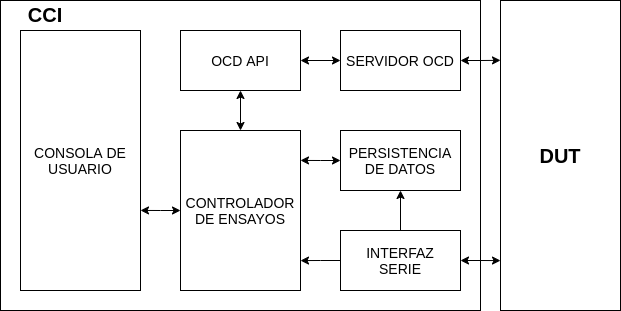
\includegraphics[width=\textwidth]{./Figuras/CCIbloques.png}
	\caption{Diagrama en bloques del Inyector por consola de comando (CCI).}
	\label{fig:diagInyector}
\end{figure}

El segundo módulo del proyecto es el firmware de autocomprobación.
En la figura \ref{fig:diagSelfTesting} se puede observar el diagrama en bloques propuesto.
Como se puede ver, este recurso deberá: verificar el estado de los periféricos, construir un informe y enviar los reportes para su análisis.

\begin{figure}[htpb]
	\centering 
	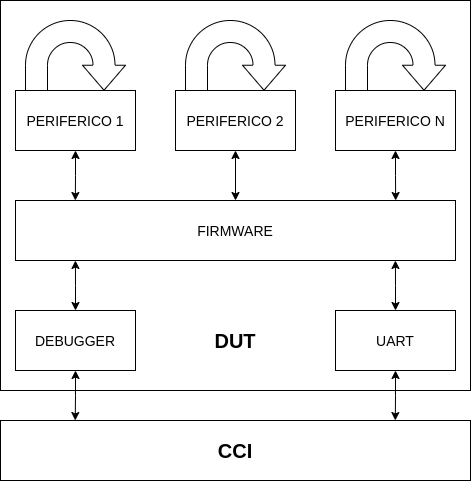
\includegraphics[width=0.8\textwidth]{./Figuras/DUTbloques.png}
	\caption{Diagrama en bloques del Proceso de dispositivo bajo prueba (DUT).}
	\label{fig:diagSelfTesting}
\end{figure}

Se espera que el proyecto agregue valor al INVAP de las siguientes maneras:

\begin{itemize}
	\item Simulando de forma acelerada la duración de una misión espacial.
	\item Permitiendo presupuestar nuevo hardware para las misiones futuras.
\end{itemize}

\section{2. Identificación y análisis de los interesados}
\label{sec:interesados}

\begin{table}[ht]
%\caption{Identificación de los interesados}
%\label{tab:interesados}
\begin{tabularx}{\linewidth}{@{}|l|X|X|l|@{}}
\hline
\rowcolor[HTML]{C0C0C0} 
Rol           & Nombre y Apellido & Organización 	& Puesto 	\\ \hline
Cliente       & \clientename      &\empclientename	& Ingeniero \\ \hline
Orientador    & Ing. Roberto Cibils & INVAP & Ingeniero \\ \hline
Responsable   & \authorname       & FIUBA        	& Alumno 	\\ \hline
Usuario final & Gerencia de Ingeniería y Producción &\empclientename	& -       	\\ \hline
\end{tabularx}
\end{table}

\begin{itemize}
	\item Cliente: es además el co-director del proyecto.
	\item Orientador: cumple el rol de usuario final.
\end{itemize}

\section{3. Propósito del proyecto}
\label{sec:proposito}

El propósito de este proyecto es proporcionar herramientas para:

\begin{itemize}
	\item Medir el nivel de susceptibilidad del software que se ejecuta en el DUT a los efectos de la radiación.
	\item Evaluar el origen de dicha susceptibilidad.
	\item Comparar la efectividad de distintas estrategias de mitigación incorporadas al software del DUT para mitigar los efectos de la radiación.
	\item Obtener la figura de mérito (FOM) del DUT.
	\item Simular los efectos del ambiente espacial en un microcontrolador.
	\item Evaluar si un dispositivo del mercado masivo puede ser utilizado en futuras misiones.
\end{itemize}

\section{4. Alcance del proyecto}
\label{sec:alcance}

El proyecto incluye en su alcance la creación de:
\begin{itemize}
	\item Un sistema de inyección de \emph{soft-errors} controlado por consola de comandos.
	\item Un firmware de autocomprobación de periféricos para el microcontrolador seleccionado por INVAP.
	\item La ejecución de ensayos de \emph{soft-errors} con la finalidad de validar el proyecto.
\end{itemize}

El presente proyecto no incluye:

\begin{itemize}
	\item El diseño de ensayos de \emph{soft-errors}.
\end{itemize}


\section{5. Supuestos del proyecto}
\label{sec:supuestos}

Para el desarrollo del presente proyecto se supone que:

\begin{itemize}
	\item Se tendrá acceso irrestricto al microcontrolador propuesto por INVAP antes del día 01/01/2022.
\end{itemize}


\section{6. Requerimientos}
\label{sec:requerimientos}

Para comprender los requerimientos del proyecto, se enumeran las siguientes definiciones, acrónimos y abreviaturas:

\begin{enumerate}
	\item Definiciones:
	\begin{itemize}
		\item Single event effect: efecto de una partícula enérgicamente cargada sobre un microcontrolador.
		\item Single event functional interrupt: interrupción causada por el impacto de una sola partícula que conduce a una no funcionalidad temporal.
		\item Single event upset: pulso transitorio en la lógica o circuitos de apoyo. Son \emph{soft-errors} no destructivos.
		\item Soft-error: tipo de error en donde una señal o dato es incorrecto.
	\end{itemize}
	\item Acrónimos:
	\begin{itemize}
		\item API: interfaz de programación de aplicaciones.
		\item DUT: dispositivo bajo prueba (microcontrolador).
		\item FOM: figura de mérito.
		\item IEEE: Instituto de Ingenieros Eléctricos y Electrónicos.
		\item OCD: on-chip debugger.
		\item SEE: single event effect.
		\item SEFI: single event functional interrupt.
		\item SEU: single event upset.
		\item TBD: a ser determinado.
		\item UART: universal asynchronous receiver-trasmitter.
	\end{itemize}
	\item Abreviaturas:
	\begin{itemize}
		\item Std: estándar.
	\end{itemize}
\end{enumerate}

A continuación se enumeran los requerimientos del proyecto según lo especificado en el estándar IEEE Std. 830-1998:

\subsection{Interfaces externas}
\label{sub:interfacesExternas}

\begin{enumerate}
	\item CCI:
	\begin{enumerate}
		\item Con usuario:
		\begin{itemize}
			\item Deberá representar todos los caracteres de ISO Std. 10646.
			\item Conformará con las secuencias de escape de ISO Std. 6429.
			\item Usará el castellano como idioma conforme a la Real Academia Española.
			\item Se aceptarán barbarismos que conformen la interfaz con los sistemas UNIX.
			\item No deberá producir destellos ni cambios bruscos en su intensidad lumínica.
			\item No deberá producir sonidos.
			\item Títulos:
			\begin{itemize}
				\item Los títulos deberán tener una longitud máxima de 30 caracteres.
				\item Los títulos deberán estar correctamente capitalizados.
				\item Los títulos deberán ser únicos.
			\end{itemize}
			\item Comandos:
			\begin{itemize}
				\item El sistema se iniciará con el comando ``sise''.
				\item El sistema imprimirá en pantalla un manual de ayuda con el comando ``sise --help''.
				\item Se podrá exportar la configuración del último ensayo realizado con el comando ``sise --export=Ruta''.
				\item Se podrá importar la configuración de un ensayo a realizar con el comando ``sise --import=Ruta/Archivo''.
			\end{itemize}
			\item Menú:
			\begin{itemize}
				\item El sistema de menú tendrá una arquitectura de árbol.
				\item La navegación entre los nodos del menú será consistente en todo el árbol.
				\item Se indicará en todo momento el nodo actual y todos los nodos que lleven a la raíz del árbol.
			\end{itemize}
		\end{itemize}
		\item Con DUT:
		\begin{itemize}
			\item La comunicación con UART será en 9600 baudios, 8 bits de datos, 1 bit de parada y 0 bits de paridad.
			\item La comunicación con el debugger se conformará con la configuración recomendada por el fabricante.
		\end{itemize}
	\end{enumerate}
	\item Proceso de DUT:
	\begin{itemize}
		\item La comunicación con el debugger estará disponible durante todo el flujo de la secuencia.
		\item Durante el flujo de la secuencia, la UART solo podrá transmitir información.
		\item En el periodo entre secuencias, la UART podrá recibir y transmitir información.
	\end{itemize}
\end{enumerate}

\subsection{Funciones}
\label{sub:funciones}

\begin{enumerate}
	\item CCI:
	\begin{itemize}
		\item Detendrá la secuencia de duración $ T $ del DUT en un momento $ t $ definido como \\ $ t \, \epsilon \, \rm I\!R^+ \wedge t \, < T$.
		\item Con la secuencia del DUT detenida, inyectará un SEFI-SEU que invertirá el valor de un bit de un registro interno.
		\item La descripción del ensayo definirá el momento $ t $ de inyección de SEFI-SEU durante la secuencia de duración $ T $ y será un múltiplo de $\Delta t$ definido como $ \Delta t=T/N \, \forall \, N \epsilon \, \rm I\!N $.
		\item La descripción del ensayo definirá la cantidad $ M $ de registros involucrados en la prueba.
		\item La cantidad de secuencias $ L $ a ejecutar quedará definida como $ L = N \times M $.
		\item Se ejecutará una secuencia de control sin inyección de SEFI-SEU antes de correr las $ L $ secuencias.
		\item Por cada ejecución de una secuencia se obtendrá un valor de salida $ S $ del DUT.
		\item Cada valor de salida $ S $ será persistido para su análisis.
		\item Cada valor de salida $ S $ quedará asociado a su correspondiente secuencia con su inyección de SEFI-SEU y momento $ t $.
		\item Se generará un archivo de resultados llamado\\ ``resultados-AAAAMMDDHHmm.res'', siendo AAAA el año del ensayo, MM el mes, DD el día, HH la hora y mm los minutos.
		\item El archivo de resultados acumulará los SEFI y SEU de cada registro del DUT.
		\item El archivo de resultados acumulará los SEU de cada periférico del DUT.
		\item El archivo de resultados indicará el FOM del registro definido como: \\
		$ FOM_{REG} = (1 - \frac{SEU}{SEFI}) $.
		\item El archivo de resultados indicará el FOM del DUT definido como: \\
		$ FOM_{DUT} = \frac{1}{M} \times \sum_{i = 1}^{i = M}FOM_{i} $ siendo $ i $ el número que representa un registro del DUT.
		\item Se generará un archivo de histogramas llamado ``histogramas-AAAAMMDDmm.his'' siendo AAAA el año del ensayo, MM el mes, DD el día, HH la hora y mm los minutos.
		\item El archivo de histogramas tendrá una tabla que indique la frecuencia de fallos como función de los SEFIs por registro del DUT.
		\item El archivo de histogramas tendrá una tabla que indique la frecuencia de fallos como función de los SEFIs por periférico del DUT.
	\end{itemize}
	\item Proceso de DUT:
	\begin{itemize}
		\item Deberá correr una secuencia de autoevaluación cuya ejecución durará un tiempo $ T $.
		\item Deberá producir una salida $ S $ que podrá ser un estado o una secuencia de estados.
		\item Este proceso podrá tener una entrada $ E $.
		\item Deberá evaluar el estado de los periféricos del DUT.
		\item Tendrá una función de evaluación para cada uno de los periféricos del DUT.
		\item Se podrá definir por la entrada $ E $ si se desea excluir uno o más periféricos en la secuencia.
		\item Manejará una interrupción del flujo normal de la secuencia y generará una salida $ S $ indicando la excepción, por ejemplo: interrupción por \emph{watchdog}.
		\item La salida $ S $ utilizará la UART del DUT para ser transmitida.
		\item La entrada $ E $ utilizará la UART del DUT para ser recibida.
	\end{itemize}
\end{enumerate}

\subsection{Requisitos de rendimiento}
\label{sub:rendimiento}

\begin{itemize}
	\item La inyección de SEFI-SEU podrá tener un desvío en su momento $ t $ de 10 ms.
	\item El desvío tolerado de $ t $ deberá representar como máximo el 1\% de la duración $ T $ de la secuencia del DUT.
	\item Aceptará un $ \Delta t $ que como mínimo represente el 5\% de la duración $ T $ de la secuencia del DUT.
\end{itemize}

\subsection{Restricciones de diseño}
\label{sub:restriccionesDiseño}

\begin{itemize}
	\item Se utilizará como dispositivo principal el microcontrolador seleccionado por INVAP.
	\item Se utilizará un sistema operativo de tiempo real para diseñar el Proceso de DUT.
\end{itemize}

\subsection{Atributos del sistema}
\label{sub:atributos}

\begin{enumerate}
	\item Mantenibilidad:
	\begin{itemize}
		\item El Proceso de DUT se desarrollará con un modelo de capas.
	\end{itemize}
\end{enumerate}

Los requerimientos mencionados se detallan en el documento SISE-RS.

\section{7. Historias de usuarios (\textit{Product backlog})}
\label{sec:backlog}

En esta sección se muestran dos historias de usuarios y su puntaje.
El puntaje es una estimación del esfuerzo necesario para cumplir una historia.
Para determinar la dificultad se consideran los siguientes factores:

\begin{itemize}
	\item Complejidad ciclomática esperada antes del \emph{refactoring}.
	\item Cantidad de módulos necesarios.
	\item Funciones que necesiten correr en tiempo real.
	\item Dificultad para implementar \emph{TDD} o \emph{BDD}.
\end{itemize}

El puntaje se expresa como un número primo entre 1 y 29.
Entonces, existen 10 puntajes posibles.
Sin embargo, una sucesión de números primos propone una escala no lineal.
Finalmente, el número 1 corresponde a una historia trivial mientras que 29 se asigna a aquella que demande el máximo esfuerzo.

A continuación se enumeran las dos historias de usuario:

\begin{itemize}
	\item Como \emph{ingeniero de desarrollo} quiero \emph{simular} los años previstos para una misión espacial en un periodo de 24 hs para \emph{evaluar} las técnicas de mitigación de errores empleadas. \emph{Story points: 7}, la historia de usuario requiere introducir \emph{soft-errors} con una frecuencia proporcional al ensayo.
	\item Como \emph{ingeniero de desarrollo} quiero \emph{obtener} la figura de mérito del microcontrolador seleccionado para \emph{decidir} si el dispositivo es adecuado para la misión. \emph{Story points: 29}, la historia de usuario requiere realizar múltiples secuencias de autovalidación con inyecciones de \emph{soft-errors} precisas.
\end{itemize}


\section{8. Entregables principales del proyecto}
\label{sec:entregables}

Los entregables del proyecto son:

\begin{itemize}
	\item Código fuente en el repositorio con control de versiones \emph{Gitlab} de INVAP.
	\item Documentación del código con \emph{Doxygen}.
	\item Documentación de las actividades semanales.
\end{itemize}


\section{9. Desglose del trabajo en tareas}
\label{sec:wbs}

\begin{enumerate}
\item Planificación
	\begin{enumerate}
	\item Investigación de la problemática (10 hs).
	\item Relevamiento de las necesidades del cliente (15 hs).
	\item Exploración de las posibles tecnologías a emplear (20 hs).
	\item Investigación sobre el nivel de acceso posible al microcontrolador (5 hs).
	\item Creación del documento de especificaciones de requerimientos de software (15 hs).
	\item Elección final de las tecnologías e informe de justificación (15 hs).
	\item Confección de un documento de planificación del proyecto (20 hs).
	\item Reunión de control y aceptación de la documentación (1 hs).
	\item Creación del plan de pruebas y validación (20 hs).
	\item Reunión final de la planificación (1 hs).
	\end{enumerate}
\item Logística e infraestructura
	\begin{enumerate}
	\item Establecimiento de un canal cifrado con el departamento de IT de INVAP (2 hs).
	\item Obtención de credenciales para acceder a la infraestructura de INVAP (2 hs).
	\item Obtención de credenciales para acceder al sistema de control de versiones de INVAP (2 hs).
	\item Configuración del entorno de trabajo conforme a los lineamientos de INVAP (3 hs).
	\item Obtención del hardware necesario para la realización del proyecto (10 hs).
	\end{enumerate}
\item Inyector por consola de comando
	\begin{enumerate}
	\item Integración del servidor OCD (10 hs).
	\item Creacion de los archivos de configuración para el servidor OCD (30 hs).
	\item Pruebas de integración servidor OCD-Dispositivo bajo prueba (10 hs).
	\item Pruebas de rendimiento del servidor OCD (10 hs).
	\item Determinación de la media y desvío del error temporal de SEFI-SEU (5 hs).
	\item Creación de API para el servidor OCD (20 hs).
	\item Pruebas de aceptación de API para el servidor OCD (10 hs).
	\item Determinación y comparación de la media y desvío del error temporal de SEFI-SEU (5 hs).
	\item Servicio de interfaz serie para el dispositivo bajo prueba (20 hs).
	\item Pruebas de rendimiento de la interfaz serie (5 hs).
	\item Servicio de persistencia de datos (20 hs).
	\item Pruebas de aceptación del servicio de persistencia de datos (5 hs).
	\item Codificación del controlador de ensayos (40 hs).
	\item Pruebas del controlador de ensayos (10 hs).
	\item Validación manual de los informes generados (10 hs).
	\item Creación de la consola de usuario (15 hs).
	\item Creación de pruebas automáticas para la consola de usuario (10 hs).
	\item Validación de la consola de usuario por parte del cliente (5 hs).
	\end{enumerate}
\item Proceso en DUT
	\begin{enumerate}
		\item Diseño de la estrategia de autovalidación del estado general del DUT (25 hs).
		\item Diseño de la estrategia de la validación del estado de cada periférico (30 hs).
		\item Análisis de los posibles SEFI-SEU que alteren la secuencia de autovalidación general (25 hs).
		\item Diseño de estrategias de manejo de excepciones (25 hs).
		\item Reunión de control y aceptación del diseño (1 hs).
		\item Codificación del firmware (50 hs).
		\item Pruebas de manejo de excepciones (25 hs).
	\end{enumerate}
\item Procesos de cierre
	\begin{enumerate}
		\item Pruebas automáticas de todo el sistema (6 hs).
		\item Obtención de la figura de mérito del microcontrolador evaluado (1 hs).
		\item Creación de la memoria del trabajo terminado (20 hs).
		\item Creación de la presentación para la defensa pública (5 hs).
		\item Creación del video para la defensa pública (5 hs).
		\item Defensa pública (0,5 hs).
		\item Agradecimiento a todos los involucrados (0,5 hs).
	\end{enumerate}
\end{enumerate}

Cantidad total de horas: (600 hs).

\section{10. Diagrama de Activity On Node}
\label{sec:AoN}

En esta sección se muestra la dependencia entre las taréas que figuran en la sección \ref{sec:wbs}.
Las tareas se agrupan en: planificación, logística e infraestructura, inyector por consola de comando, proceso en DUT y procesos de cierre.
En la figura \ref{fig:AoN} se puede observar la suceción de las categorías.
Además, se indica con la variable ``T'' la cantidad de horas que consume cada grupo.
Finalmente en las figuras \ref{fig:AoN1}, \ref{fig:AoN2}, \ref{fig:AoN3}, \ref{fig:AoN4} y \ref{fig:AoN5}; se muestran las tareas que forman parte de cada categoría.

\begin{figure}[htpb]
\centering 

\tikzstyle{startEnd}=[draw,ultra thick, fill=black!10, text width=5em, text centered, minimum height=5em, circle]
\tikzstyle{normalTask}=[draw, text width=8em, text centered, minimum height=8em]
\tikzstyle{criticalTask}=[draw,ultra thick, fill=black!10, text width=8em, text centered, minimum height=8em]	
\tikzstyle{invisible}=[text width=8em, text centered, minimum height=5em]
\begin{tikzpicture}[align=center,node distance=4.5cm]
\node(inicio) [startEnd] {INICIO 24/06/21};
\node[below of=inicio] (aux) [invisible] {};
\node[left of=aux] (w1) [criticalTask] {1. Planificación. $T=102$};
\node[right of=aux] (w2) [normalTask] {2. Logística e infraestructura. $T=102$};
\node[below of=w1] (w3) [normalTask] {3. Inyector por consola de comando. $T=85$};
\node[right of=w3] (w4) [criticalTask] {4. Proceso en DUT. $T=181$};
\node[below of=w4] (w5) [criticalTask] {5. Procesos de cierre. $T=38$};
\node[below of=w5] (fin) [startEnd] {FIN 15/05/22};

\draw[-{Latex[length=3mm]},ultra thick] (inicio)-|(w1);
\draw[-{Latex[length=3mm]}] (inicio)-|(w2);
\draw[-{Latex[length=3mm]}] (w2)|-(w5);
\draw[-{Latex[length=3mm]}] (w1)--(w3);
\draw[-{Latex[length=3mm]},ultra thick] (w1)-|(w4);
\draw[-{Latex[length=3mm]},ultra thick] (w4)--(w5);
\draw[-{Latex[length=3mm]}] (w3)|-(w5);
\draw[-{Latex[length=3mm]},ultra thick] (w5)--(fin);
\end{tikzpicture}

\caption{Diagrama en \textit{Activity on Node}.}
\label{fig:AoN}
\end{figure}

\begin{figure}[htpb]
	\centering 
	\tikzstyle{normalTask}=[draw, text width=8em, text centered, minimum height=8em]
	\tikzstyle{criticalTask}=[draw,ultra thick, fill=black!10, text width=8em, text centered, minimum height=8em]	
	\begin{tikzpicture}[align=center,node distance=4.5cm]
	
	\node (n1) [criticalTask] {1.1 Investigación de la problemática. $T=10$};
	\node [below of=n1] (n2) [criticalTask] {1.2 Relevamiento de las necesidades del cliente. $T=15$};
	
	\node [left of=n2] (n3) [criticalTask] {1.3 Exploración de las posibles tecnologías a emplear. $T=20$};
	\node [right of=n2] (n4) [normalTask] {1.4 Investigación sobre el nivel de acceso posible al DUT. $T=20$};
	
	\node [below of=n2] (n7) [criticalTask] {1.7 Confección de un documento de planificación del proyecto. $T=20$};
	\node [left of=n7] (n6) [criticalTask] {1.6 Elección de tecnologías e informe de justificación. $T=15$};
	\node [right of=n7] (n5) [normalTask] {1.5 Especificaciones de requerimientos de software. $T=15$};
	
	\node[below of=n7] (n8) [criticalTask] {1.8 Reunión de control y aceptación de la documentación. $T=1$};
	\node[right of=n8] (n9) [criticalTask] {1.9 Creación del plan de pruebas y validación. $T=20$};
	\node[below of=n9] (n10) [criticalTask] {1.10 Reunión final de la planificación. $T=1$};
	
	\node[left of=n10] (n11) [criticalTask] {Planificación finalizada};
	
	\draw[-{Latex[length=3mm]},ultra thick] (n1)--(n2);
	
	\draw[-{Latex[length=3mm]},ultra thick] (n2)--(n3);
	\draw[-{Latex[length=3mm]}] (n2)--(n4);
	
	\draw[-{Latex[length=3mm]}] (n4)--(n5);
	\draw[-{Latex[length=3mm]}] (n5)--(n7);
	\draw[-{Latex[length=3mm]},ultra thick] (n3)--(n6);
	\draw[-{Latex[length=3mm]},ultra thick] (n6)--(n7);
	
	\draw[-{Latex[length=3mm]},ultra thick] (n7)--(n8);
	\draw[-{Latex[length=3mm]},ultra thick] (n8)--(n9);
	\draw[-{Latex[length=3mm]},ultra thick] (n9)--(n10);
	
	\draw[-{Latex[length=3mm]},ultra thick] (n10)--(n11);
	\end{tikzpicture}
	
	\caption{Diagrama en \textit{Activity on Node}: planificación.}
	\label{fig:AoN1}
\end{figure}

\begin{figure}[htpb]
	\centering 
	\tikzstyle{normalTask}=[draw, text width=8em, text centered, minimum height=8em]
	\tikzstyle{criticalTask}=[draw,ultra thick, fill=black!10, text width=8em, text centered, minimum height=8em]	
	\begin{tikzpicture}[align=center,node distance=5cm]
	
	\node(n1) [criticalTask] {2.1 Establecimiento de un canal cifrado con el dpto. de IT INVAP. $T=2$};
	\node[right of=n1] (n2) [criticalTask] {2.2 Credenciales para acceder a la infraestructura de INVAP. $T=2$};
	\node[below of=n2] (n3) [criticalTask] {2.3 Credenciales para acceder al SCV de INVAP. $T=2$};
	\node[left of=n3] (n4) [criticalTask] {2.4 Configuración de entrono de trabajo (INVAP). $T=3$};
	\node[below of=n4] (n5) [criticalTask] {2.5 Obtención del hardware necesario para la realización del proyecto. $T=10$};
	\node[right of=n5] (n6) [criticalTask] {Fin de logística e infraestructura};
	
	\draw[-{Latex[length=3mm]},ultra thick] (n1)--(n2);
	\draw[-{Latex[length=3mm]},ultra thick] (n2)--(n3);
	\draw[-{Latex[length=3mm]},ultra thick] (n3)--(n4);
	\draw[-{Latex[length=3mm]},ultra thick] (n4)--(n5);
	\draw[-{Latex[length=3mm]},ultra thick] (n5)--(n6);
	
	\end{tikzpicture}
	\caption{Diagrama en \textit{Activity on Node}: logística e infraestructura.}
	\label{fig:AoN2}
\end{figure}

\begin{figure}[htpb]
	\centering 
	\tikzstyle{startEnd}=[draw,ultra thick, fill=black!10, text width=4em, text centered, minimum height=5em, circle]
	\tikzstyle{normalTask}=[draw, text width=5.5em, text centered, minimum height=6em]
	\tikzstyle{criticalTask}=[draw,ultra thick, fill=black!10, text width=5.5em, text centered, minimum height=6em]	
	\begin{tikzpicture}[align=center,node distance=2.7cm]
	\node(s)[startEnd]{Inicio};
	\node[right of=s](n2)[criticalTask]{\footnotesize{3.2 Creación de archivos de configuración OCD. $T=30$}};
	\node[below of=n2](n1)[criticalTask]{\footnotesize{3.1 Integración del servidor OCD. $T=10$}};
	\node[below of=n1](n9)[normalTask]{\footnotesize{3.9 Servicio de interfaz serie para el DUT. $T=20$}};
	\node[below of=n9](n11)[normalTask]{\footnotesize{3.11 Servicio de persistencia de datos. $T=20$}};
	\node[below of=n11](n13)[normalTask]{\footnotesize{3.13 Creación: controlador de ensayos. $T=40$}};
	\node[below of=n13](n16)[normalTask]{\footnotesize{3.16 Creación de la consola de usuario. $T=15$}};
	
	\node[right of=n2](n3)[criticalTask]{\footnotesize{3.3 Pruebas de integración OCD-DUT. $T=10$}};
	\node[right of=n1](n6)[criticalTask]{\footnotesize{3.6 Creación de API OCD. $T=20$}};
	\node[right of=n9](n10)[normalTask]{\footnotesize{3.10 Pruebas de rendimiento: interfaz serie. $T=5$}};
	\node[right of=n11](n12)[normalTask]{\footnotesize{3.12 Pruebas de aceptación: persistencia de datos. $T=5$}};
	\node[right of=n13](n14)[normalTask]{\footnotesize{3.14 Pruebas: controlador de ensayos. $T=10$}};
	\node[right of=n16](n17)[normalTask]{\footnotesize{3.17 Creación de pruebas: consola de usuario. $T=10$}};
	
	\node[right of=n3](n4)[normalTask]{\footnotesize{3.4 Pruebas de rendimiento: servidor OCD. $T=10$}};
	\node[right of=n6](n7)[criticalTask]{\footnotesize{3.7 Pruebas de aceptación: servidor OCD. $T=10$}};
	\node[right of=n14](n15)[normalTask]{\footnotesize{3.15 Validar informes generados. $T=10$}};
	\node[right of=n17](n18)[normalTask]{\footnotesize{3.18 Validación: consola de usuario. $T=5$}};
	
	\node[right of=n4](n5)[normalTask]{\footnotesize{3.5 Media y desvío temporal SEFI-SEU. $T=5$}};
	\node[right of=n7](n8)[criticalTask]{\footnotesize{3.8 Media y desvío temporal SEFI-SEU. $T=5$}};
	
	\node[right of=n8](fin)[criticalTask]{\footnotesize{Fin: inyector por consola de comando}};
	
	\draw[-{Latex[length=3mm]}] (s)|-(n16);
	\draw[-{Latex[length=3mm]}] (s)|-(n13);
	\draw[-{Latex[length=3mm]}] (s)|-(n11);
	\draw[-{Latex[length=3mm]}] (s)|-(n9);
	\draw[-{Latex[length=3mm]},ultra thick] (s)|-(n1);
	\draw[-{Latex[length=3mm]},ultra thick] (n1)--(n2);
	
	\draw[-{Latex[length=3mm]},ultra thick] (n2)--(n3);
	\draw[-{Latex[length=3mm]},ultra thick] (n3)--(n6);
	\draw[-{Latex[length=3mm]}] (n9)--(n10);
	\draw[-{Latex[length=3mm]}] (n11)--(n12);
	\draw[-{Latex[length=3mm]}] (n13)--(n14);
	\draw[-{Latex[length=3mm]}] (n16)--(n17);
	
	\draw[-{Latex[length=3mm]}] (n3)--(n4);
	\draw[-{Latex[length=3mm]},ultra thick] (n6)--(n7);
	\draw[-{Latex[length=3mm]}] (n14)--(n15);
	\draw[-{Latex[length=3mm]}] (n17)--(n18);
	
	\draw[-{Latex[length=3mm]}] (n4)--(n5);
	\draw[-{Latex[length=3mm]},ultra thick] (n7)--(n8);
	
	\draw[-{Latex[length=3mm]}] (n5)-|(fin);
	\draw[-{Latex[length=3mm]},ultra thick] (n8)--(fin);
	\draw[-{Latex[length=3mm]}] (n10)-|(fin);
	\draw[-{Latex[length=3mm]}] (n12)-|(fin);
	\draw[-{Latex[length=3mm]}] (n15)-|(fin);
	\draw[-{Latex[length=3mm]}] (n18)-|(fin);
	
	\end{tikzpicture}
	\caption{Diagrama en \textit{Activity on Node}: inyector por consola de comando.}
	\label{fig:AoN3}
\end{figure}

\begin{figure}[htpb]
	\centering 
	\tikzstyle{normalTask}=[draw, text width=8em, text centered, minimum height=7em]
	\tikzstyle{criticalTask}=[draw,ultra thick, fill=black!10, text width=8em, text centered, minimum height=7em]	
	\begin{tikzpicture}[align=center,node distance=4cm]
	
	\node(n1) [criticalTask] {4.1 Diseño de autovalidación de estado del DUT. $T=25$};
	\node[right of=n1] (n2) [criticalTask] {4.2 Diseño de validación de periféricos. $T=30$};
	\node[below of=n2] (n3) [criticalTask] {4.3 Análisis de SEFI-SEU que alteren la secuencia. $T=25$};
	\node[left of=n3] (n4) [criticalTask] {4.4 Estrategias de manejo de excepciones. $T=25$};
	\node[below of=n4] (n5) [criticalTask] {4.5 Reunión de control y aceptación. $T=1$};
	\node[right of=n5] (n6) [criticalTask] {4.6 Creación del firmware. $T=50$};
	\node[below of=n6] (n7) [criticalTask] {4.7 Pruebas: manejo de excepciones. $T=25$};
	\node[left of=n7] (n8) [criticalTask] {Fin: proceso en DUT};
	
	\draw[-{Latex[length=3mm]},ultra thick] (n1)--(n2);
	\draw[-{Latex[length=3mm]},ultra thick] (n2)--(n3);
	\draw[-{Latex[length=3mm]},ultra thick] (n3)--(n4);
	\draw[-{Latex[length=3mm]},ultra thick] (n4)--(n5);
	\draw[-{Latex[length=3mm]},ultra thick] (n5)--(n6);
	\draw[-{Latex[length=3mm]},ultra thick] (n6)--(n7);
	\draw[-{Latex[length=3mm]},ultra thick] (n7)--(n8);
	
	\end{tikzpicture}
	\caption{Diagrama en \textit{Activity on Node}: proceso en DUT.}
	\label{fig:AoN4}
\end{figure}

\begin{figure}[htpb]
	\centering 
	\tikzstyle{startEnd}=[draw,ultra thick, fill=black!10, text width=4em, text centered, minimum height=5em, circle]
	\tikzstyle{normalTask}=[draw, text width=8em, text centered, minimum height=7em]
	\tikzstyle{criticalTask}=[draw,ultra thick, fill=black!10, text width=8em, text centered, minimum height=7em]	
	\begin{tikzpicture}[align=center,node distance=4cm]
	
	\node(n1) [criticalTask] {5.1 Pruebas automáticas de todo el sistema. $T=6$};
	\node[right of=n1] (n2) [criticalTask] {5.2 Obtención del FOM del DUT. $T=1$};
	\node[below of=n2] (n3) [criticalTask] {5.3 Creación de la memoria del trabajo. $T=20$};
	\node[left of=n3] (n4) [criticalTask] {5.4 Creación de la presentación para la defensa pública. $T=5$};
	\node[below of=n4] (n5) [criticalTask] {5.5 Creación del vídeo para la defensa pública. $T=5$};
	\node[right of=n5] (n6) [criticalTask] {5.6 Defensa pública. $T=0.5$};
	\node[below of=n6] (n7) [criticalTask] {5.7 Agradecimiento a todos los involucrados. $T=0.5$};
	\node[left of=n7] (n8) [startEnd] {Fin};
	
	\draw[-{Latex[length=3mm]},ultra thick] (n1)--(n2);
	\draw[-{Latex[length=3mm]},ultra thick] (n2)--(n3);
	\draw[-{Latex[length=3mm]},ultra thick] (n3)--(n4);
	\draw[-{Latex[length=3mm]},ultra thick] (n4)--(n5);
	\draw[-{Latex[length=3mm]},ultra thick] (n5)--(n6);
	\draw[-{Latex[length=3mm]},ultra thick] (n6)--(n7);
	\draw[-{Latex[length=3mm]},ultra thick] (n7)--(n8);
	
	\end{tikzpicture}
	\caption{Diagrama en \textit{Activity on Node}: procesos de cierre.}
	\label{fig:AoN5}
\end{figure}

\begin{landscape}
	
\section{11. Diagrama de Gantt}
\label{sec:gantt}

A partir de los diagramas en \emph{Activity On Node} de la sección \ref{sec:AoN} se creó un diagrama de gantt. Se lo puede observar en las figuras \ref{fig:gantt1}, \ref{fig:gantt2}, \ref{fig:gantt3}, \ref{fig:gantt4}, \ref{fig:gantt5}, \ref{fig:gantt6}, \ref{fig:gantt7} y \ref{fig:gantt8}.

\begin{figure}[htbp]
\begin{center}
\newgantttimeslotformat{stardate}{%
	\def\decomposestardate##1.##2\relax{%
		\def\stardateyear{##1}\def\stardateday{##2}%
	}%
\decomposestardate#1\relax%
\pgfcalendardatetojulian{\stardateyear-01-01}{#2}%
\advance#2 by-1\relax%
\advance#2 by\stardateday\relax%
}
\begin{ganttchart}[
	hgrid,
	vgrid,
	time slot format=stardate
	]{2021.174}{2021.210}
	\gantttitlecalendar{year, month=name, day} \\
	\ganttgroup{1 PLANIFICACIÓN}{2021.175}{2021.210} \\
	\ganttbar{1.1 Investigación de la problemática}{2021.175}{2021.178} \ganttnewline
	\ganttbar{1.2 Relevamiento de las necesidades}{2021.179}{2021.182} \ganttnewline
	\ganttbar{1.3 Exploración de las tecnologías}{2021.183}{2021.189} \ganttnewline
	\ganttbar{1.4 Investigación: acceso DUT}{2021.190}{2021.193} \ganttnewline
	\ganttbar{1.5 Especificación de requerimientos}{2021.194}{2021.197} \ganttnewline
	\ganttbar{1.6 Elección final de tecnologías}{2021.198}{2021.210}
	\ganttlink{elem1}{elem2}
	\ganttlink{elem2}{elem3}
	\ganttlink{elem3}{elem4}
	\ganttlink{elem4}{elem5}
	\ganttlink{elem5}{elem6}
\end{ganttchart}
\end{center}
\caption{Diagrama de gantt: parte 1.}
\label{fig:gantt1}
\end{figure}

\end{landscape}

\begin{landscape}

\begin{figure}[htbp]
	\begin{center}
		\newgantttimeslotformat{stardate}{%
			\def\decomposestardate##1.##2\relax{%
				\def\stardateyear{##1}\def\stardateday{##2}%
			}%
			\decomposestardate#1\relax%
			\pgfcalendardatetojulian{\stardateyear-01-01}{#2}%
			\advance#2 by-1\relax%
			\advance#2 by\stardateday\relax%
		}
		\begin{ganttchart}[
			hgrid,
			vgrid,
			time slot format=stardate
			]{2021.218}{2021.254}
			\gantttitlecalendar{year, month=name, day} \\
			\ganttgroup{1 PLANIFICACIÓN}{2021.218}{2021.232} \\
			\ganttbar{1.6 Elección final de tecnologías}{2021.218}{2021.219} \ganttnewline
			\ganttbar{1.7 Planificación del proyecto}{2021.220}{2021.226} \ganttnewline
			\ganttbar{1.8 Reunión de control}{2021.227}{2021.227} \ganttnewline
			\ganttbar{1.9 Plan de pruebas y validación}{2021.228}{2021.232} \ganttnewline
			\ganttbar{1.10 Reunión final de la planificación}{2021.232}{2021.232} \ganttnewline
			\ganttmilestone{FIN PLANIFICACIÓN}{2021.232} \ganttnewline
			\ganttgroup{2 INFRAESTRUCTURA}{2021.233}{2021.240} \\
			\ganttbar{2.1 Canal IT de INVAP}{2021.233}{2021.235} \ganttnewline
			\ganttbar{2.2 Credenciales de VLAN de INVAP}{2021.235}{2021.235} \ganttnewline
			\ganttbar{2.3 Credenciales de Gitlab de INVAP}{2021.236}{2021.236} 
			\ganttlink{elem1}{elem2}
			\ganttlink{elem2}{elem3}
			\ganttlink{elem3}{elem4}
			\ganttlink{elem4}{elem5}
			\ganttlink{elem5}{elem6}
			\ganttlink{elem6}{elem8}
			\ganttlink{elem8}{elem9}
			\ganttlink{elem9}{elem10}
		\end{ganttchart}
	\end{center}
	\caption{Diagrama de gantt: parte 2.}
	\label{fig:gantt2}
\end{figure}

\end{landscape}

\begin{landscape}
	
	\begin{figure}[htbp]
		\begin{center}
			\newgantttimeslotformat{stardate}{%
				\def\decomposestardate##1.##2\relax{%
					\def\stardateyear{##1}\def\stardateday{##2}%
				}%
				\decomposestardate#1\relax%
				\pgfcalendardatetojulian{\stardateyear-01-01}{#2}%
				\advance#2 by-1\relax%
				\advance#2 by\stardateday\relax%
			}
			\begin{ganttchart}[
				hgrid,
				vgrid,
				time slot format=stardate
				]{2021.236}{2021.272}
				\gantttitlecalendar{year, month=name, day} \\
				\ganttgroup{2 INFRAESTRUCTURA}{2021.236}{2021.240} \\
				\ganttbar{2.4 Entorno de trabajo}{2021.236}{2021.236} \ganttnewline
				\ganttbar{2.5 Obtención del hardware}{2021.237}{2021.240} \ganttnewline
				\ganttmilestone{FIN INFRAESTRUCTURA}{2021.240} \ganttnewline
				\ganttgroup{3 CCI}{2021.241}{2021.272} \\
				\ganttbar{3.1 Integración del servidor OCD}{2021.241}{2021.243} \ganttnewline
				\ganttbar{3.2 Configuración del servidor OCD}{2021.244}{2021.253} \ganttnewline
				\ganttbar{3.3 Pruebas de integración OCD}{2021.254}{2021.257} \ganttnewline
				\ganttbar{3.4 Pruebas de rendimiento OCD}{2021.258}{2021.260} \ganttnewline
				\ganttbar{3.5 Determinación de error temporal}{2021.261}{2021.263} \ganttnewline
				\ganttbar{3.6 API para el servidor OCD}{2021.264}{2021.270}
				\ganttlink{elem1}{elem2}
				\ganttlink{elem2}{elem3}
				\ganttlink{elem3}{elem5}
				\ganttlink{elem5}{elem6}
				\ganttlink{elem6}{elem7}
				\ganttlink{elem7}{elem8}
				\ganttlink{elem8}{elem9}
				\ganttlink{elem9}{elem10}
			\end{ganttchart}
		\end{center}
		\caption{Diagrama de gantt: parte 3.}
		\label{fig:gantt3}
	\end{figure}
	
\end{landscape}

\begin{landscape}
	
	\begin{figure}[htbp]
		\begin{center}
			\newgantttimeslotformat{stardate}{%
				\def\decomposestardate##1.##2\relax{%
					\def\stardateyear{##1}\def\stardateday{##2}%
				}%
				\decomposestardate#1\relax%
				\pgfcalendardatetojulian{\stardateyear-01-01}{#2}%
				\advance#2 by-1\relax%
				\advance#2 by\stardateday\relax%
			}
			\begin{ganttchart}[
				hgrid,
				vgrid,
				time slot format=stardate
				]{2021.271}{2021.307}
				\gantttitlecalendar{year, month=name, day} \\
				\ganttgroup{3 CCI}{2021.271}{2021.307} \\
				\ganttbar{3.7 Aceptación de la API OCD}{2021.271}{2021.273} \ganttnewline
				\ganttbar{3.8 Error temporal SEFI-SEU}{2021.274}{2021.274} \ganttnewline
				\ganttbar{3.9 Interfaz serie}{2021.275}{2021.280} \ganttnewline
				\ganttbar{3.10 Rendimiento interfaz serie}{2021.281}{2021.284} \ganttnewline
				\ganttbar{3.11 Persistencia de datos}{2021.285}{2021.291} \ganttnewline
				\ganttbar{3.12 Pruebas de persistencia de datos}{2021.292}{2021.292} \ganttnewline
				\ganttbar{3.13 Controlador de ensayos}{2021.293}{2021.306} \ganttnewline
				\ganttbar{3.14 Pruebas controlador de ensayos}{2021.307}{2021.307}
				\ganttlink{elem1}{elem2}
				\ganttlink{elem2}{elem3}
				\ganttlink{elem3}{elem4}
				\ganttlink{elem4}{elem5}
				\ganttlink{elem5}{elem6}
				\ganttlink{elem6}{elem7}
				\ganttlink{elem7}{elem8}
			\end{ganttchart}
		\end{center}
		\caption{Diagrama de gantt: parte 4.}
		\label{fig:gantt4}
	\end{figure}
	
\end{landscape}

\begin{landscape}
	
	\begin{figure}[htbp]
		\begin{center}
			\newgantttimeslotformat{stardate}{%
				\def\decomposestardate##1.##2\relax{%
					\def\stardateyear{##1}\def\stardateday{##2}%
				}%
				\decomposestardate#1\relax%
				\pgfcalendardatetojulian{\stardateyear-01-01}{#2}%
				\advance#2 by-1\relax%
				\advance#2 by\stardateday\relax%
			}
			\begin{ganttchart}[
				hgrid,
				vgrid,
				time slot format=stardate
				]{2021.309}{2021.345}
				\gantttitlecalendar{year, month=name, day} \\
				\ganttgroup{3 CCI}{2021.309}{2021.324} \\
				\ganttbar{3.14 Pruebas controlador de ensayos}{2021.309}{2021.309} \ganttnewline
				\ganttbar{3.15 Validación de informes generados}{2021.310}{2021.313} \ganttnewline
				\ganttbar{3.16 Creación de consola de usuario}{2021.314}{2021.319} \ganttnewline
				\ganttbar{3.17 Pruebas de consola de usuario}{2021.320}{2021.322} \ganttnewline
				\ganttbar{3.18 Validación de consola de usuario}{2021.323}{2021.324} \ganttnewline
				\ganttmilestone{FIN CCI}{2021.324} \ganttnewline
				\ganttgroup{4 PROCESO EN DUT}{2021.325}{2021.345} \\
				\ganttbar{4.1 Autovalidación general}{2021.325}{2021.333} \ganttnewline
				\ganttbar{4.2 Autovalidación de periféricos}{2021.334}{2021.343} \ganttnewline
				\ganttbar{4.3 Análisis SEFI-SEU}{2021.344}{2021.345}
				\ganttlink{elem1}{elem2}
				\ganttlink{elem2}{elem3}
				\ganttlink{elem3}{elem4}
				\ganttlink{elem4}{elem5}
				\ganttlink{elem5}{elem6}
				\ganttlink{elem6}{elem8}
				\ganttlink{elem8}{elem9}
				\ganttlink{elem9}{elem10}
			\end{ganttchart}
		\end{center}
		\caption{Diagrama de gantt: parte 5.}
		\label{fig:gantt5}
	\end{figure}
	
\end{landscape}

\begin{landscape}
	
	\begin{figure}[htbp]
		\begin{center}
			\newgantttimeslotformat{stardate}{%
				\def\decomposestardate##1.##2\relax{%
					\def\stardateyear{##1}\def\stardateday{##2}%
				}%
				\decomposestardate#1\relax%
				\pgfcalendardatetojulian{\stardateyear-01-01}{#2}%
				\advance#2 by-1\relax%
				\advance#2 by\stardateday\relax%
			}
			\begin{ganttchart}[
				hgrid,
				vgrid,
				time slot format=stardate
				]{2021.350}{2022.21}
				\gantttitlecalendar{year, month=name, day} \\
				\ganttgroup{4 PROCESO EN DUT}{2021.350}{2022.21} \\
				\ganttbar{4.3 Análisis SEFI-SEU}{2021.350}{2021.351} \ganttnewline
				\ganttbar{4.4 Manejo de excepciones}{2021.352}{2021.361} \ganttnewline
				\ganttbar{4.5 Reunión de control y aceptación}{2021.362}{2021.362} \ganttnewline
				\ganttbar{4.6 Codificación del firmware}{2021.362}{2022.13} \ganttnewline
				\ganttbar{4.7 Pruebas de manejo de excepciones}{2022.14}{2022.21} \ganttnewline
				\ganttmilestone{FIN PROCESO EN DUT}{2022.21}
				\ganttlink{elem1}{elem2}
				\ganttlink{elem2}{elem3}
				\ganttlink{elem3}{elem4}
				\ganttlink{elem4}{elem5}
			\end{ganttchart}
		\end{center}
		\caption{Diagrama de gantt: parte 6.}
		\label{fig:gantt6}
	\end{figure}
	
\end{landscape}

\begin{landscape}
	
	\begin{figure}[htbp]
		\begin{center}
			\newgantttimeslotformat{stardate}{%
				\def\decomposestardate##1.##2\relax{%
					\def\stardateyear{##1}\def\stardateday{##2}%
				}%
				\decomposestardate#1\relax%
				\pgfcalendardatetojulian{\stardateyear-01-01}{#2}%
				\advance#2 by-1\relax%
				\advance#2 by\stardateday\relax%
			}
			\begin{ganttchart}[
				hgrid,
				vgrid,
				time slot format=stardate
				]{2022.22}{2022.58}
				\gantttitlecalendar{year, month=name, day} \\
				\ganttgroup{5 PROCESOS DE CIERRE}{2022.22}{2022.58} \\
				\ganttbar{5.1 Pruebas de todo el sistema}{2022.22}{2022.25} \ganttnewline
				\ganttbar{5.2 Figura de mérito DUT}{2022.26}{2022.26} \ganttnewline
				\ganttbar{5.3 Memoria del trabajo terminado}{2022.27}{2022.37} \ganttnewline
				\ganttbar{5.4 Presentación para defensa}{2022.38}{2022.41} \ganttnewline
				\ganttbar{5.5 Vídeo para defensa}{2022.42}{2022.45}
				\ganttlink{elem1}{elem2}
				\ganttlink{elem2}{elem3}
				\ganttlink{elem3}{elem4}
				\ganttlink{elem4}{elem5}
			\end{ganttchart}
		\end{center}
		\caption{Diagrama de gantt: parte 7.}
		\label{fig:gantt7}
	\end{figure}
	
\end{landscape}

\begin{landscape}
	
	\begin{figure}[htbp]
		\begin{center}
			\newgantttimeslotformat{stardate}{%
				\def\decomposestardate##1.##2\relax{%
					\def\stardateyear{##1}\def\stardateday{##2}%
				}%
				\decomposestardate#1\relax%
				\pgfcalendardatetojulian{\stardateyear-01-01}{#2}%
				\advance#2 by-1\relax%
				\advance#2 by\stardateday\relax%
			}
			\begin{ganttchart}[
				hgrid,
				vgrid,
				time slot format=stardate
				]{2022.152}{2022.188}
				\gantttitlecalendar{year, month=name, day} \\
				\ganttgroup{5 PROCESOS DE CIERRE}{2022.152}{2022.175} \\
				\ganttbar{5.6 Defensa pública}{2022.175}{2022.175} \ganttnewline
				\ganttbar{5.7 Agradecimiento a los involucrados}{2022.175}{2022.175} \ganttnewline
				\ganttmilestone{FIN}{2022.175}
				\ganttlink{elem1}{elem2}
				\ganttlink{elem2}{elem3}
			\end{ganttchart}
		\end{center}
		\caption{Diagrama de gantt: parte 8.}
		\label{fig:gantt8}
	\end{figure}
	
\end{landscape}


\section{12. Presupuesto detallado del proyecto}
\label{sec:presupuesto}

\begin{table}[htpb]
\centering
\begin{tabularx}{\linewidth}{@{}|X|c|r|r|@{}}
\hline
\rowcolor[HTML]{C0C0C0} 
\multicolumn{4}{|c|}{\cellcolor[HTML]{C0C0C0}COSTOS DIRECTOS} \\ \hline
\rowcolor[HTML]{C0C0C0} 
Descripción &
  \multicolumn{1}{c|}{\cellcolor[HTML]{C0C0C0}Cantidad} &
  \multicolumn{1}{c|}{\cellcolor[HTML]{C0C0C0}Valor unitario} &
  \multicolumn{1}{c|}{\cellcolor[HTML]{C0C0C0}Valor total} \\ \hline
 Dispositivo bajo prueba (DUT)&
  \multicolumn{1}{c|}{1} &
  \multicolumn{1}{c|}{USD 50} &
  \multicolumn{1}{c|}{USD 50} \\ \hline
 Honorarios del ingeniero &
  \multicolumn{1}{c|}{1} &
  \multicolumn{1}{c|}{USD 0} &
  \multicolumn{1}{c|}{USD 0} \\ \hline
\multicolumn{1}{|l|}{} &
   &
   &
   \\ \hline
\multicolumn{1}{|l|}{} &
   &
   &
   \\ \hline
\multicolumn{3}{|c|}{SUBTOTAL} &
  \multicolumn{1}{c|}{USD 50} \\ \hline
\rowcolor[HTML]{C0C0C0} 
\multicolumn{4}{|c|}{\cellcolor[HTML]{C0C0C0}COSTOS INDIRECTOS} \\ \hline
\rowcolor[HTML]{C0C0C0} 
Descripción &
  \multicolumn{1}{c|}{\cellcolor[HTML]{C0C0C0}Cantidad} &
  \multicolumn{1}{c|}{\cellcolor[HTML]{C0C0C0}Valor unitario} &
  \multicolumn{1}{c|}{\cellcolor[HTML]{C0C0C0}Valor total} \\ \hline
\multicolumn{1}{|l|}{} &
   &
   &
   \\ \hline
\multicolumn{1}{|l|}{} &
   &
   &
   \\ \hline
\multicolumn{1}{|l|}{} &
   &
   &
   \\ \hline
\multicolumn{3}{|c|}{SUBTOTAL} &
  \multicolumn{1}{c|}{} \\ \hline
\rowcolor[HTML]{C0C0C0}
\multicolumn{3}{|c|}{TOTAL} &
   \\ \hline
\end{tabularx}%
\end{table}


\section{13. Gestión de riesgos}
\label{sec:riesgos}

Riesgo 1: Demora en la adquisición del DUT.
\begin{itemize}
	\item Severidad (S): 5.\\
	Las tareas asociadas al proceso en DUT están en el camino crítico.
	\item Probabilidad de ocurrencia (O): 5.\\
	El proveedor declara una demora estimada de 5 meses de entrega. No es posible saber la exactitud de la estimación.
\end{itemize}   

Riesgo 2: Destrucción del DUT durante un ensayo.
\begin{itemize}
	\item Severidad (S): 10. \\
	Se demorarían 5 meses en reponer el DUT.
	\item Ocurrencia (O): 2. \\
	No se espera someter al DUT a ensayos potencialmente destructivos.
\end{itemize}

Riesgo 3: Avería del ordenador de desarrollo.
\begin{itemize}
	\item Severidad (S): 3. \\
	El código generado se mantiene en repositorios con control de versiones.
	\item Ocurrencia (O): 2. \\
	El ordenador de desarrollo es robusto, se encuentra en una posición fija y tiene elementos de protección eléctrica.
\end{itemize}

Riesgo 4: Disminución de las horas disponibles.
\begin{itemize}
	\item Severidad (S): 6. \\
	El proyecto fue planificado con 20 horas de trabajo semanal.
	\item Ocurrencia (O): 2. \\
	Las horas de trabajo fueron ubicadas en los días no laborables del tesista.
\end{itemize}

Riesgo 5: Imposibilidad económica para continuar el posgrado.
\begin{itemize}
	\item Severidad (S): 10. \\
	La consecuencia sería el fin del proyecto.
	\item Ocurrencia (O): 1. \\
	Se cuenta con el suficiente ahorro para afrontar los costos.
\end{itemize}

b) Tabla de gestión de riesgos:      (El RPN se calcula como RPN=SxO)

\begin{table}[htpb]
\centering
\begin{tabularx}{\linewidth}{@{}|X|c|c|c|c|c|c|@{}}
\hline
\rowcolor[HTML]{C0C0C0} 
Riesgo                                             & S & O & RPN & S* & O* & RPN* \\ \hline
Demora en la adquisición del DUT                   & 5 & 5 & 25  &3   & 5  & 15   \\ \hline
Destrucción del DUT durante un ensayo              &10 & 2 & 20  &10  & 1  & 10   \\ \hline
Avería del ordenador de desarrollo                 & 3 & 2 & 6   &    &    &      \\ \hline
Disminución de las horas disponibles               & 6 & 2 & 12  &    &    &      \\ \hline
Imposibilidad económica para continuar el posgrado &10 & 1 & 10  &    &    &      \\ \hline
\end{tabularx}%
\end{table}

Criterio adoptado: 
Se tomarán medidas de mitigación en los riesgos cuyos números de RPN sean mayores a 19.

Nota: los valores marcados con (*) en la tabla corresponden luego de haber aplicado la mitigación.

c) Plan de mitigación de los riesgos que originalmente excedían el RPN máximo establecido:
 
Riesgo 1: uso de un modelo alternativo al DUT. \\
  - Severidad (S): 3. \\
  El modelo alternativo permite avanzar con parte del proyecto mientras se espera el arribo del DUT. \\
  - Probabilidad de ocurrencia (O): 5. \\
  No hay modificación en la probabilidad de ocurrencia.

Riesgo 2: aprobación del plan de ensayos por parte del director y co-director. \\
  - Severidad (S): 10. \\
  No hay modificación en la severidad. \\
  - Probabilidad de ocurrencia (O): 5. \\
  El apoyo del director y co-director incrementan las posibilidades de detectar una acción potencialmente destructiva.

\section{14. Gestión de la calidad}
\label{sec:calidad}

\begin{itemize} 
\item Req \#1: Deberá representar todos los caracteres de ISO Std. 10646.
\begin{itemize}
	\item Verificación: construcción de una pantalla de prueba de caracteres.
	\item Validación: aceptación de la pantalla de prueba por parte del cliente.  
\end{itemize}

\item Req \#2: Conformará con las secuencias de escape de ISO Std. 6429.
\begin{itemize}
    \item Verificación: construcción de una pantalla de prueba de secuencias de escape.
    \item Validación: aceptación de la pantalla de prueba por parte del cliente.
\end{itemize}

\item Req \#3: Usará el castellano como idioma conforme a la Real Academia Española.
\begin{itemize}
    \item Verificación: los mensajes a mostrar en pantalla serán contruidos a partir de un ``template'' que será analizado por un corrector ortográfico.
    \item Validación: aceptación del idioma por parte del cliente.
\end{itemize}

\item Req \#4: Se aceptarán barbarismos que conformen la interfaz con los sistemas UNIX.
\begin{itemize}
    \item Verificación: se usarán los comandos en inglés que se utilizan en los programas GNU.
    \item Validación: aceptación de los comandos por parte del cliente.
\end{itemize}

\item Req \#5: No deberá producir destellos ni cambios bruscos en su intensidad lumínica.
\begin{itemize}
    \item Verificación: no se utilizarán las secuencias de escape que generen destellos en la terminal.
    \item Validación: se realizarán las pruebas de funcionamiento del sistema en un cuarto con total oscuridad y se reportará cualquier síntoma de fotofobia.
\end{itemize}

\item Req \#6: No deberá producir sonidos.
\begin{itemize}
    \item Verificación: no se utilizarán las secuencias de escape que generen sonidos en la terminal.
    \item Validación: se realizarán las pruebas de funcionamiento del sistema con el control de volumen al máximo y se reportará cualquier sonido emitido.
\end{itemize}

\item Req \#7: Los títulos deberán tener una longitud máxima de 30 caracteres.
\begin{itemize}
    \item Verificación: ningún título superará los 30 caracteres.
    \item Validación: aceptación de los títulos por parte del cliente.
\end{itemize}

\item Req \#8: Los títulos deberán estar correctamente capitalizados.
\begin{itemize}
    \item Verificación: se generará una biblioteca que imponga el formato de los títulos.
    \item Validación: aceptación de los títulos por parte del cliente.
\end{itemize}

\item Req \#9: Los títulos deberán ser únicos.
\begin{itemize}
    \item Verificación: los títulos se cargarán en memoria en una colección del tipo ``set''.
    \item Validación: aceptación de los títulos por parte del cliente.
\end{itemize}

\item Req \#10: El sistema se iniciará con el comando ``sise''.
\begin{itemize}
    \item Verificación: se utilizará ``setuptools\_entry\_points'' para crear un comando en el ``path'' del ambiente.
    \item Validación: se creará una maqueta que ejecutará el cliente en su ambiente de produción.
\end{itemize}

\item Req \#11: El sistema imprimirá en pantalla un manual de ayuda con el comando ``sise --help''.
\begin{itemize}
    \item Verificación: se utilizará ``setuptools\_entry\_points'' para crear un comando ``--help'' como argumento de ``sise''.
    \item Validación: se creará una maqueta que ejecutará el cliente en su ambiente de producción.
\end{itemize}

\item Req \#12: Se podrá exportar la configuración del último ensayo realizado con el comando ``sise --export=Ruta''.
\begin{itemize}
    \item Verificación: se utilizará ``setuptools\_entry\_points'' para crear un comando \\``--export=Ruta'' como argumento de ``sise''.
    \item Validación: se creará una maqueta que ejecutará el cliente en su ambiente de producción.
\end{itemize}

\item Req \#13: Se podrá importar la configuración de un ensayo a realizar con el comando ``sise --import=Ruta/Archivo''.
\begin{itemize}
    \item Verificación: se utilizará ``setuptools\_entry\_points'' para crear un comando \\``--import=Ruta/Archivo'' como argumento de ``sise''.
    \item Validación: se creará una maqueta que ejecutará el cliente en su ambiente de producción.
\end{itemize}

\item Req \#14: El sistema de menú tendrá una arquitectura de árbol.
\begin{itemize}
    \item Verificación: se recorrerá el menú y se intentará ingresar a una rama inaccesible.
    \item Validación: aceptación del menú por parte del cliente.
\end{itemize}

\item Req \#15: La navegación entre los nodos del menú será consistente en todo el árbol.
\begin{itemize}
    \item Verificación: se recorrerá el menú y se reportará cualquier inconsistencia encontrada.
    \item Validación: aceptación del menú por parte del cliente.
\end{itemize}

\item Req \#16: Se indicará en todo momento el nodo actual y todos los nodos que lleven a la raíz del árbol.
\begin{itemize}
    \item Verificación: se recorrerá el menú y se reportará cualquier nodo que rompa la cadena de información.
    \item Validación: aceptación del menú por parte del cliente.
\end{itemize}

\item Req \#17: La comunicación con UART será en 9600 baudios, 8 bits de datos, 1 bit de parada y 0 bits de paridad.
\begin{itemize}
    \item Verificación: se utilizará una terminal serie con la configuración del requerimiento para verificar la comunicación.
    \item Validación: se utilizará el DUT para validar la comunicación.
\end{itemize}

\item Req \#18: La comunicación con el debugger se conformará con la configuración recomendada por el fabricante.
\begin{itemize}
    \item Verificación: Se generará un guión para probar la comunicación con el debugger.
    \item Validación: Se realizará una prueba que modifique el registro PC del DUT y deberá modificar el normal funcionamiento de un programa de prueba.
\end{itemize}

\item Req \#19: La comunicación con el debugger estará disponible durante todo el flujo de la secuencia.
\begin{itemize}
    \item Verificación: se generará un guión que verifique la conexión del servidor OCD con el debugger durante toda la secuencia del DUT.
    \item Validación: se realizará una prueba continua de 24 horas de duración y no se deberá perder la comunicación.
\end{itemize}

\item Req \#20: Durante el flujo de la secuencia, la UART solo podrá transmitir información.
\begin{itemize}
    \item Verificación: se creará un script que intentará comunicarse con el DUT durante la secuencia.
    \item Validación: análisis con \emph{wireshark} para validar que no existe comunicación serie.
\end{itemize}

\item Req \#21: En el periodo entre secuencias, la UART podrá recibir y transmitir información.
\begin{itemize}
    \item Verificación: se creará un script que intentará comunicarse con el DUT entre secuencias.
    \item Validación: análisis con \emph{wireshark} para validar la comunicación serie.
\end{itemize}

\item Req \#22: Detendrá la secuencia de duración $ T $ del DUT en un momento $ t $ definido como \\ $ t \, \epsilon \, \rm I\!R^+ \wedge t \, < T$.
\begin{itemize}
    \item Verificación: se contará la cantidad de instrucciones desde el inicio de la secuencia hasta el momento $ t $ y se calculará el tiempo transcurrido.
    \item Validación: se generará una secuencia de duración $ T $ que encienda un LED al finalizar. El instante $ t $ deberá suceder antes del encendido del testigo.
\end{itemize}

\item Req \#23: Con la secuencia del DUT detenida, inyectará un SEFI-SEU que invertirá el valor de un bit de un registro interno.
\begin{itemize}
    \item Verificación: se utilizará el módulo \emph{Coresight} de la arquitectura ARM para verificar la inyección del SEFI-SEU.
    \item Validación: se modificará el valor del registro \emph{program counter} y se deberá observar un cambio en el comportamiento del DUT.
\end{itemize}

\item Req \#24: La descripción del ensayo definirá el momento $ t $ de inyección de SEFI-SEU durante la secuencia de duración $ T $ y será un múltiplo de $\Delta t$ definido como $ \Delta t=T/N \, \forall \, N \epsilon \, \rm I\!N $
\begin{itemize}
    \item Verificación: se contará la cantidad de instrucciones entre inyecciones de SEFI-SEU y el número deberá ser constante.
    \item Validación: se deberán producir $ N $ inyecciones de SEFI-SEU.
\end{itemize}

\item Req \#25: La descripción del ensayo definirá la cantidad $ M $ de registros involucrados en la prueba.
\begin{itemize}
    \item Verificación: se comparará la cantidad de registros incluidos en la descripción del ensayo con la cantidad de registros especificados en las hojas de datos.
    \item Validación: se comparará los registros incluidos en el ensayo con la especificación de la arquitectura ARM.
\end{itemize}

\item Req \#26: La cantidad de secuencias $ L $ a ejecutar quedará definida como $ L = N \times M $.
\begin{itemize}
    \item Verificación: Se contará la cantidad de mensajes recibidos y deberá ser igual a $ L $.
    \item Validación: La cantidad de muestras que alimentan al histograma deberá ser $ L $.
\end{itemize}

\item Req \#27: Se ejecutará una secuencia de control sin inyección de SEFI-SEU antes de correr las $ L $ secuencias.
\begin{itemize}
    \item Verificación: El mensaje recibido luego de la ejecución de la primera secuencia no tendrá errores.
    \item Validación: La primera secuencia tendrá una duración $ T $.
\end{itemize}

\item Req \#28: Por cada ejecución de una secuencia se obtendrá un valor de salida $ S $ del DUT.
\begin{itemize}
    \item Verificación: Se deberá obtener una cantidad $ L $ de salidas $ S $.
    \item Validación: Los datos persistidos deberán tener una cantidad $ L $ de salidas $ S $.
\end{itemize}

\item Req \#29: Cada valor de salida $ S $ será persistido para su análisis.
\begin{itemize}
    \item Verificación: Se deberá obtener una cantidad $ L $ de salidas $ S $.
    \item Validación: Los datos persistidos deberán tener una cantidad $ L $ de salidas $ S $.
\end{itemize}

\item Req \#30: Cada valor de salida $ S $ quedará asociado a su correspondiente secuencia con su inyección de SEFI-SEU y momento $ t $.
\begin{itemize}
    \item Verificación: se observará la tabla de datos creada y no podrán quedar celdas vacías.
    \item Validación: Los datos persistidos deberán tener una cantidad $ L $ de salidas $ S $.
\end{itemize}

\item Req \#31: Se generará un archivo de resultados llamado\\ ``resultados-AAAAMMDDHHmm.res'', siendo AAAA el año del ensayo, MM el mes, DD el día, HH la hora y mm los minutos.
\begin{itemize}
    \item Verificación: se generará archivos y se comparará los nombres obtenidos con el reloj del sistema.
    \item Validación: se observará que los archivos tengan el patrón especificado.
\end{itemize}

\item Req \#32: El archivo de resultados acumulará los SEFI y SEU de cada registro del DUT.
\begin{itemize}
    \item Verificación: se utilizará \emph{wireshark} para contar las salidas $ S $ y deberá coincidir con la acumulación de SEFI-SEU.
    \item Validación: se repetirá el ensayo múltiples veces y los resultados acumulados deberan coincidir.
\end{itemize}

\item Req \#33: El archivo de resultados acumulará los SEU de cada periférico del DUT.
\begin{itemize}
    \item Verificación: la cantidad de SEFI-SEU obtenidos por registró deberá coincidir con los SEFI-SEU obtenidos por periféricos.
    \item Validación: la cantidad de SEFI-SEU obtenidos por registró deberá coincidir con los SEFI-SEU obtenidos por periféricos.
\end{itemize}

\item Req \#34: El archivo de resultados indicará el FOM del registro definido como: \\ $ FOM_{REG} = (1 - \frac{SEU}{SEFI}) $.
\begin{itemize}
    \item Verificación: se realizará una verificación automática con pytest del cálculo de FOM.
    \item Validación: el FOM obtenido será un número entre 0 y 1.
\end{itemize}

\item Req \#35: El archivo de resultados indicará el FOM del DUT definido como: \\ $ FOM_{DUT} = \frac{1}{M} \times \sum_{i = 1}^{i = M}FOM_{i} $ siendo $ i $ el número que representa un registro del DUT.
\begin{itemize}
    \item Verificación: se realizará una verificación automática con pytest del cálculo de FOM.
    \item Validación: el FOM obtenido será un número entre 0 y 1.
\end{itemize}

\item Req \#36: Se generará un archivo de histogramas llamado\\ ``histogramas-AAAAMMDDmm.his'' siendo AAAA el año del ensayo, MM el mes, DD el día, HH la hora y mm los minutos.
\begin{itemize}
    \item Verificación: se generará archivos y se comparará los nombres obtenidos con el reloj del sistema.
    \item Validación: se observará que los archivos tengan el patrón especificado.
\end{itemize}

\item Req \#37: El archivo de histogramas tendrá una tabla que indique la frecuencia de fallos como función de los SEFIs por registro del DUT.
\begin{itemize}
    \item Verificación: se verificará con \emph{wireshark} que la cantidad de fallos reportados sea la misma que la informada en el archivo de histogramas.
    \item Validación: la cantidad total de fallas no podrá superar el número $ L $.
\end{itemize}

\item Req \#38: El archivo de histogramas tendrá una tabla que indique la frecuencia de fallos como función de los SEFIs por periférico del DUT.
\begin{itemize}
    \item Verificación: se verificará con \emph{wireshark} que la cantidad de fallos reportados sea la misma que la informada en el archivo de histogramas.
    \item Validación: la cantidad total de fallas no podrá superar el número $ L $.
\end{itemize}

\item Req \#39: Deberá correr una secuencia de autoevaluación cuya ejecución durará un tiempo $ T $.
\begin{itemize}
    \item Verificación: se usará la cuenta de instrucciones del core para medir el tiempo $ T $.
    \item Validación: se usará el reloj del sistema para medir el tiempo $ T $.
\end{itemize}

\item Req \#40: Deberá producir una salida $ S $ que podrá ser un estado o una secuencia de estados.
\begin{itemize}
    \item Verificación: se usará \emph{wireshark} para verificar la salida $ S $.
    \item Validación: se usará una terminal serie para validar la salida $ S $.
\end{itemize}

\item Req \#41: Este proceso podrá tener una entrada $ E $.
\begin{itemize}
    \item Verificación:
    \item Validación:
\end{itemize}

\item Req \#42: Deberá evaluar el estado de los periféricos del DUT.
\begin{itemize}
    \item Verificación: se crearán procesos en DUT que generen fallas en todos los periféricos para verificar la evaluación.
    \item Validación: se desconectaran los loops externos de los periféricos, generando fallas en todos ellos.
\end{itemize}

\item Req \#43: Tendrá una función de evaluación para cada uno de los periféricos del DUT.
\begin{itemize}
    \item Verificación: se forzará la falla de todos los periféricos.
    \item Validación: se compararan los informes con la lista de periféricos de las hojas de datos del DUT.
\end{itemize}

\item Req \#44: Se podrá definir por la entrada $ E $ si se desea excluir uno o más periféricos en la secuencia.
\begin{itemize}
    \item Verificación: se verificará con \emph{wireshark} que los periféricos excluidos no sean reportados.
    \item Validación: se validará con los informes generados que los periféricos excluidos no sean reportados.
\end{itemize}

\item Req \#45: Manejará una interrupción del flujo normal de la secuencia y generará una salida $ S $ indicando la excepción, por ejemplo: interrupción por \emph{watchdog}.
\begin{itemize}
    \item Verificación: se forzará la falla recurrente de un periférico en particular para verificar que todas las salidas $ S $.
    \item Validación: se observará el informe generado para validar que la cantidad de salidas $ S $ sea igual a $ L $.
\end{itemize}

\item Req \#46: La salida $ S $ utilizará la UART del DUT para ser transmitida.
\begin{itemize}
    \item Verificación: se utilizará \emph{wireshark} para verificar la salida $ S $.
    \item Validación: se utilizará una terminal serie para validar la salida $ S $.
\end{itemize}

\item Req \#47: La entrada $ E $ utilizará la UART del DUT para ser recibida.
\begin{itemize}
    \item Verificación: se utilizará \emph{wireshark} para verificar la entrada $ E $.
    \item Validación: se utilizará una terminal serie para enviar entradas $ E $.
\end{itemize}

\item Req \#48: La inyección de SEFI-SEU podrá tener un desvío en su momento $ t $ de 10 ms.
\begin{itemize}
    \item Verificación: se medirá la cantidad de instrucciones ejecutadas para calcular el error del momento $ t $.
    \item Validación: se utilizará el reloj del sistema para calcular el error del momento $ t $.
\end{itemize}

\item Req \#49: El desvío tolerado de $ t $ deberá representar como máximo el 1\% de la duración $ T $ de la secuencia del DUT.
\begin{itemize}
    \item Verificación: se medirá la cantidad de instrucciones ejecutadas para calcular el desvío del momento $ t $.
    \item Validación: se utilizará el reloj del sistema para calcular el desvío del momento $ t $.
\end{itemize}

\item Req \#50: Aceptará un $ \Delta t $ que como mínimo represente el 5\% de la duración $ T $ de la secuencia del DUT.
\begin{itemize}
    \item Verificación: se medirá la cantidad de instrucciones ejecutadas para calcular el $ \Delta t $.
    \item Validación: se utilizará el reloj del sistema para calcular el $ \Delta t $.
\end{itemize}

\item Req \#51: Se utilizará como dispositivo principal el microcontrolador seleccionado por INVAP.
\begin{itemize}
    \item Verificación: se comparará el microcontrolador con las hojas de datos proporcionadas.
    \item Validación: el cliente confirmará que el microcontrolador es el DUT deseado.
\end{itemize}

\item Req \#52: Se utilizará un sistema operativo de tiempo real para diseñar el Proceso de DUT.
\begin{itemize}
    \item Verificación: se utilizará un RTOS reconocido en la industria.
    \item Validación: el cliente aprobará el RTOS seleccionado.
\end{itemize}

\item Req \#53: El Proceso de DUT se desarrollará con un modelo de capas.
\begin{itemize}
    \item Verificación: se generará el firmware en múltiples unidades de traducción.
    \item Validación: el director y co-director validarán la arquitectura del firmware.
\end{itemize}

\end{itemize}

\section{15. Procesos de cierre}    
\label{sec:cierre}

Establecer las pautas de trabajo para realizar una reunión final de evaluación del proyecto, tal que contemple las siguientes actividades:

\begin{itemize}
	\item Pautas de trabajo que se seguirán para analizar si se respetó el Plan de Proyecto original:
        \begin{itemize}
            \item El responsable del proyecto analizará el plan original y se verificará el grado de correspondencia con su ejecución.
            \item El responsable del proyecto evaluará las tareas que no se ajustaron al plan para detectar las causas y tenerlas en cuentas en próximos proyectos.
	    \end{itemize}

    \item Identificación de las técnicas y procedimientos útiles e inútiles que se emplearon, y los problemas que surgieron y cómo se solucionaron:
	    \begin{itemize}
            \item El responsable del proyecto evaluará la eficacia de la técnica TDD.
            \item El responsable del proyecto generará informes con todos los problemas técnicos no previstos.
        \end{itemize}
	\item Luego de la presentación del trabajo ante el jurado, el responsable del proyecto realizará un agradecimiento público a todas las personas involucradas en el proyecto. 
\end{itemize}

\end{document}
